\chapter{Additional Ablations}
\section{Additional Sampling Scheme Ablations}
\Cref{table:samplingschemesnotblobs} and \Cref{table:samplingschemesblobs} show the effect of using different sampling schemes on the BDD-Inpainting and BDD-Inpainting-Blobs test sets, respectively. The sampling schemes tested are depicted in \Cref{fig:old-sampling-schemes} and \Cref{fig:sampling-schemes}. For each metric, the best performing sampling scheme is indicated in bold font. All measurements were taken using the Heun sampler \citep{karras2022elucidating} with 100 sampling steps. The Improved AR w/ Far Future performs best on both test sets across almost all metrics. Sampling scheme ablations are omitted for Inpainting-Background and Inpainting-Cars as we found an autoregressive scheme gave significantly better qualitative results than the other schemes.
\begin{table}[h]
\centering
\caption{Effect of sampling schemes measured on the BDD-Inpainting test set.}
\label{table:samplingschemesnotblobs}
\customrescaleone{
\begin{tabular}{llllllllllllll}
\toprule
Sampling Scheme & PSNR$\blacktriangle$ & SSIM$\blacktriangle$   & LPIPS$\blacktriangledown$     & PVCS$\blacktriangledown$   & FID$\blacktriangledown$   & VFID$\blacktriangledown$   & $E_\text{warp}$$\blacktriangledown$ \\ 
\midrule
3-Res. Improved AR                                                & 32.81 & 0.9678 & 0.0289 & 0.2302 & 1.75 & 0.0884 & $2.19{\cdot}10^{\shortminus3}$ \\
Improved AR w/ Far Future                                         & 33.68 & \textbf{0.9717} & \textbf{0.0261} & \textbf{0.2037} & \textbf{1.71} & \textbf{0.0748} & $\mathbf{1.79{\cdot}10^{\shortminus3}}$ \\
AR                                                                & 32.97 & 0.9699 & 0.0278 & 0.2166 & 1.78 & 0.0778 & $1.85{\cdot}10^{\shortminus3}$ \\
Hierarchy-2                                                       & 32.96 & 0.9690 & 0.0284 & 0.2232 & 1.74 & 0.0839 & $1.97{\cdot}10^{\shortminus3}$ \\
2-Res. Improved AR                                                & 33.18 & 0.9692 & 0.0278 & 0.2201 & 1.72 & 0.0815 & $2.03{\cdot}10^{\shortminus3}$ \\
Reverse AR                                                        & \textbf{33.31} & 0.9702 & 0.0273 & 0.2132 & 1.76 & 0.0785 & $\mathbf{1.79{\cdot}10^{\shortminus3}}$ \\ 
\bottomrule
\end{tabular}}
\end{table}
\begin{table}[h]
\centering
\caption{Effect of sampling schemes measured on the BDD-Inpainting-Blobs test set.}
\label{table:samplingschemesblobs}
\customrescaleone{
\begin{tabular}{llllllllllllll}
\toprule
Sampling Scheme & PSNR$\blacktriangle$ & SSIM$\blacktriangle$   & LPIPS$\blacktriangledown$     & PVCS$\blacktriangledown$   & FID$\blacktriangledown$   & VFID$\blacktriangledown$   & $E_\text{warp}$$\blacktriangledown$ \\ 
\midrule
3-Res. Improved AR                        & 29.89 & 0.9561 & 0.0475 & 0.3142 & 1.63 & 0.1188 &  $2.00{\cdot}10^{\shortminus3}$ \\
Improved AR w/ Far Future                 & \textbf{30.67} & \textbf{0.9608} & \textbf{0.0442} & \textbf{0.2857} & 1.69 & \textbf{0.1083} &  $1.53{\cdot}10^{\shortminus3}$  \\
AR                                        & 29.45 & 0.9547 & 0.0512 & 0.3319 & 2.07 & 0.1328 &  $1.61{\cdot}10^{\shortminus3}$  \\
Hierarchy-2                               & 29.97 & 0.9570 & 0.0474 & 0.3106 & 1.65 & 0.1137 &  $1.74{\cdot}10^{\shortminus3}$  \\
2-Res. Improved AR                        & 30.25 & 0.9583 & 0.0454 & 0.2991 & \textbf{1.59} & 0.1116 &  $1.79{\cdot}10^{\shortminus3}$   \\
Reverse AR                                & 30.04 & 0.9590 & 0.0450 & 0.2920 & 1.8  & 0.1134 &  $\mathbf{1.51{\cdot}10^{\shortminus3}}$  \\
\bottomrule
\end{tabular}}
\end{table}
\section{Qualitative Sampling Scheme Ablations}
\label{sec:quall}
In this section we highlight the qualitative impact that different sampling schemes can have on the quality of inpainted videos. We select a video from the test set where conditioning on the appropriate frames is crucial for our method to succeed. \Cref{fig:qual-begin} shows the beginning of this video, where a car is occluded in the right-hand lane for the first few seconds of the video (see input frames in the first row). The Autoregressive (AR) scheme (second row) shows a distinct ``pop-in'' effect, as when the initial frames were generated the model was not able to condition on future frames where the cars existence and appearance are revealed. Both Reverse-AR and AR w/ Far Future (third and fourth rows) do condition on future frames that contain the car; Reverse-AR because the model is able to propagate the car backwards through time, and AR w/ Far Future because the model conditions on frames far out into the future where the car has been revealed. \Cref{fig:qual-end} shows the end of the video, where the cars in the right-hand lane are occluded and remain occluded for the rest of the video (first row). The AR scheme keeps these cars visible, as it is able to propagate them forward through time (second row). Reverse-Autoreg (third row) fails for the same reason that Autoreg did at the beginning: when the final frames were generated, the model was not able to condition on frames where the vehicles were visible. AR w/ Far Future (fourth row) is again successful; despite the cars not becoming visble again (and thus there is no ``future'' to condition on), it is able to propagate the cars forward in time as the Autoreg scheme does. We provide an mp4 video showing the entire inpainting for this video using the sampling schemes discussed here and more in the supplementary, with filename \texttt{appendix\_E2.mp4}. Sampling schemes used in each tile are labelled in the video.
\begin{figure*}[h!]
\begin{center}
    \centering
    \captionsetup{type=figure}
    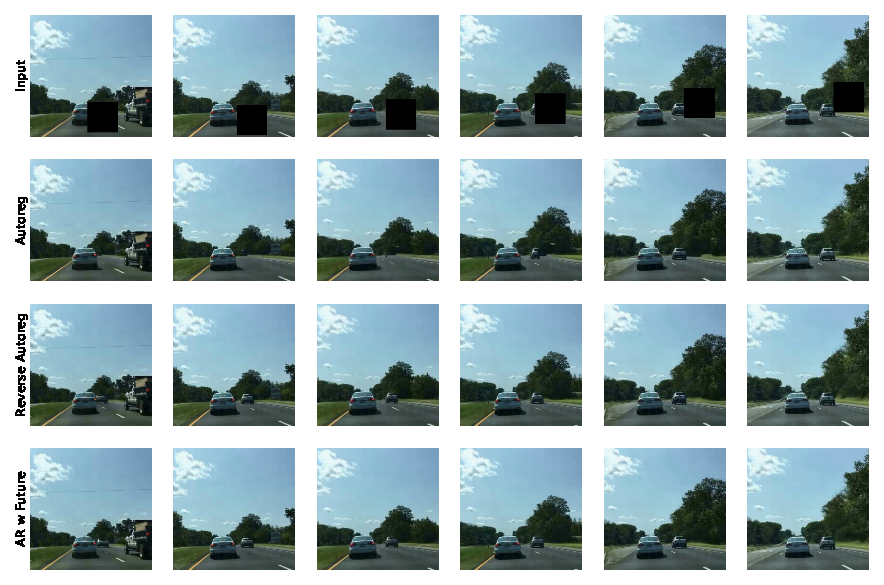
\includegraphics[width=\linewidth]{figures/james_quall/james_quall_beginning.pdf}
    \caption{Qualitative results from different sampling schemes on the beginning of the video discussed in \Cref{sec:quall}}
    \label{fig:qual-begin}
    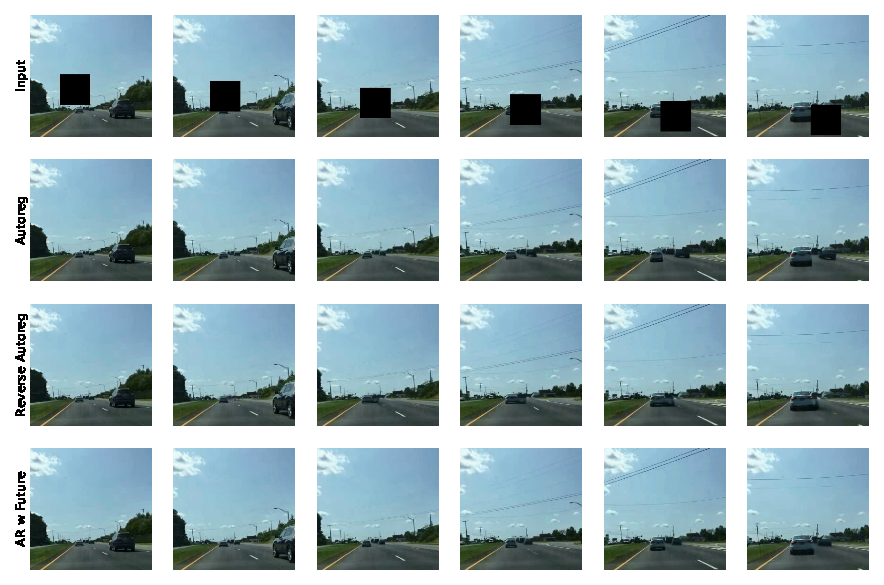
\includegraphics[width=\linewidth]{figures/james_quall/james_quall_end.pdf}
    \caption{Qualitative results from different sampling schemes on the end of the video discussed in \Cref{sec:quall}}
    \label{fig:qual-end}
\end{center}
\end{figure*}






